%%%--------------------------------%%%
%%% Domain
%%%--------------------------------%%%
\newpage
\section{Software Specification}
\label{sec:domainB}

\subsection{Purpose and Scope}
\label{sec:domainBa}
What is the software for and what is not part of the project (I'm integrating the vision part here because I don't think we need to state why we describe requirements)

\subsection{Functionalities}
\label{sec:domainBb}
Basically just the \ac{UC}

\subsubsection{Overall Use Case Diagram}
\label{sec:domainBba}


\newpage
% UC1 ====================================================
\subsubsection{Use Case Specification: \ac{UC}1 User CRUD}
\label{sec:domainBbb}

\paragraph*{Description}\mbox{}\\
Describe the functionality

\paragraph*{Screenshots}\mbox{}\\
Insert screenshots and shortly explain what can be seen
\begin{figure}[h] 
	\centering
	
\includegraphics[width=0.1\textwidth]{Content/Domain/placeholder.png}
	\caption{Use Case X: Detail}
	\label{fig:useCaseXDetailY}
\end{figure}

\paragraph*{Basic Flow} \mbox{}\\

Describe the most common path through this use case

\subparagraph{Activity Diagram}\mbox{}\\
\begin{figure}[h]
	\centering
	
\includegraphics[width=0.1\textwidth]{Content/Domain/placeholder.png}
	\caption{Activity Diagram Use Case X}
	\label{fig:activityDiagramX}
\end{figure}

\paragraph*{Alternative Flows}\mbox{}\\
What can go wrong :D

\paragraph*{Special Requirements and Preconditions}\mbox{}\\
Where does the user come from, what does he have to do before he gets here

\paragraph*{Postconditions and Persistance}\mbox{}\\
What has changed and how do we make sure the change persists?


\newpage
% UC2 ====================================================
\subsubsection{Use Case Specification: \ac{UC}2 Team Access Management CRUD}
\label{sec:domainBbc}

\paragraph*{Description}\mbox{}\\
Describe the functionality

\paragraph*{Screenshots}\mbox{}\\
Insert screenshots and shortly explain what can be seen
\begin{figure}[h] 
	\centering
	
\includegraphics[width=0.1\textwidth]{Content/Domain/placeholder.png}
	\caption{Use Case X: Detail}
	\label{fig:label1}
\end{figure}

\paragraph*{Basic Flow} \mbox{}\\

Describe the most common path through this use case

\subparagraph{Activity Diagram}\mbox{}\\
\begin{figure}[h]
	\centering
	
\includegraphics[width=0.1\textwidth]{Content/Domain/placeholder.png}
	\caption{Activity Diagram Use Case X}
	\label{fig:label11}
\end{figure}

\paragraph*{Alternative Flows}\mbox{}\\
What can go wrong :D

\paragraph*{Special Requirements and Preconditions}\mbox{}\\
Where does the user come from, what does he have to do before he gets here

\paragraph*{Postconditions and Persistance}\mbox{}\\
What has changed and how do we make sure the change persists?

\newpage
% UC3 ====================================================
\subsubsection{Use Case Specification: \ac{UC}3 Risk CRUD}
\label{sec:domainBbd}

\paragraph*{Description}\mbox{}\\
This use case allows users to create, read, update and delete risks. 
A risk consists of the following fields:
\begin{itemize}
	\vspace{-3mm}
	\setlength\itemsep{-1em}
	\item name (String)
	\item description (String)
\end{itemize}
Following fields are filled later and are not part of the input form:
\begin{itemize}
	\vspace{-3mm}
	\setlength\itemsep{-1em}
	\item probability of occurence (Enum)
	\item impact (Enum)
	\item risk factor (Enum)
	\item response (Objects)  
	\item person in charge (User)
	\item public risk (boolean)
\end{itemize}

\paragraph*{Screenshots}\mbox{}\\
tbd: Insert screenshots and shortly explain what can be seen
\begin{figure}[h] 
	\centering
	
\includegraphics[width=0.1\textwidth]{Content/Domain/placeholder.png}
	\caption{\ac{UC}3 Risk CRUD: TODO}
	\label{fig:label3}
\end{figure}

\newpage
\paragraph*{Basic Flow} \mbox{}\\
\noindent
Creating a risk:
\begin{itemize}
	\vspace{-3mm}
	\setlength\itemsep{-1.5em}
	\item  When the user clicks the "+" button at the project overview page.
	\item Then the screen for adding a new risk is opened.
	\item When the risk form is filled by the user.
	\item And the user clicks on the "Propose risk" button.
	\item Then the risk is synced with the server.
\end{itemize}

\spacing{1}
\noindent
Reading a risk:
\begin{itemize}
	\vspace{-3mm}
	\setlength\itemsep{-1em}
	\item The user is on the project overview site with all project risks.
	\item By clicking on a risk a detail risk view is opened.
	\item For exiting the risk detail view a return button ("Close" button) is clicked.
\end{itemize}

\noindent
Updating a risk: 
\begin{itemize}
	\vspace{-3mm}
	\setlength\itemsep{-1em}
	\item The user is on the project overview site with all project risks.
	\item By clicking on a risk a detail risk view is opened.
	\item On the detail view there is a pen button, enabling editing and changing the "Close" button to a "Save" button.
	\item When clicking the "Save" button the changes are syncronized with the server.
\end{itemize} 

\noindent
Deleting a risk:
\begin{itemize}
	\vspace{-3mm}
	\setlength\itemsep{-1em}
	\item The user is on the project overview site with all project risks.
	\item By clicking on a risk a detail risk view is opened.
	\item By clicking a "Delete" button the risk is deleted. This behavior is changed in UC6 Risk Discussion described in chapter \ref{sec:domainBbg}.
\end{itemize}

\spacing{1.5}
 
\subparagraph{Activity Diagram}\mbox{}\\
\begin{figure}[h]
	\centering
	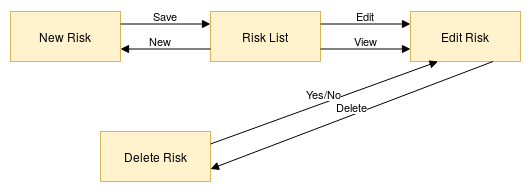
\includegraphics[width=0.9\textwidth]{Content/Domain/UC3RiskCRUDactivitydiagram.png}
	\caption{Activity Diagram \ac{UC}3 Risk CRUD}
	\label{fig:activityDiagramUC3}
\end{figure}

\paragraph*{Alternative Flows}\mbox{}\\
n/a

\paragraph*{Special Requirements and Preconditions}\mbox{}\\
The preconditions for this use case are:
\begin{enumerate}
	\vspace{-3mm}
	\setlength\itemsep{-1em}
	\item A project exists.
	\item The user is member of the project.
	\item The user has clicked the "+" button at the project overview page to add a new risk.
\end{enumerate}

\paragraph*{Postconditions and Persistance}\mbox{}\\
The postconditions for this use case are:
\begin{enumerate}
	\vspace{-3mm}
	\setlength\itemsep{-1em}
	\item The risk is immediately part of the projects risk table (this behavior is changed within UC6 Risk Discussion described in chapter \ref{sec:domainBbg}).
\end{enumerate}

\noindent
The persistence guidelines are: 
\newline
\noindent
The risk form was completely or partly filled by the user. When the user tries to leave the page now, there should be a prompt for exiting. When the risk form is filled out and the button "Propose risk" is clicked a POST request syncs the status with the server.

\newpage
% UC4 ====================================================
\subsubsection{Use Case Specification: \ac{UC}4 Project risk adjustment}
\label{sec:domainBbe}

\paragraph*{Description}\mbox{}\\
After a risk has been submitted and evaluated by the team it is grouped into three categories. However, within these categories the initial order is simply that the risks submitted first will be placed at the top. This use case allows the teams to prioritize risks according to their perceived risk urgency. On the project risk overview page the after the initial risk evaluation users will find a button they can use to adjust the ranking. They will then enter adjustment mode where they can arrange the risks according to their perceived urgency and submit their ranking. Then they will return to the overview where the risks will be displayed according to their average relative ranking positions. The adjust button will be disabled until new risks are added to prevent manipulation. The user will be notified that they cannot rank multiple times when they first go through the adjustment process. 

\paragraph*{Screenshots}\mbox{}\\
tbd: Insert screenshots and shortly explain what can be seen

\begin{figure}[h] 
	\centering
	
\includegraphics[width=0.1\textwidth]{Content/Domain/placeholder.png}
	\caption{Use Case X: Detail}
	\label{fig:label4}
\end{figure}

\paragraph*{Basic Flow} \mbox{}\\
\begin{itemize}
	\vspace{-3mm}
	\setlength\itemsep{-1em}
	\item The user is on the project overview site with all project risks.
	\item By clicking on a "Rank Risks" button the ranking view is enabled and the button becomes a submit button.
	\item The user can order the risks according to his personal priority.
	\item The user submits their preferred order.
	\item This order is submitted to the server and the average rank for every risk according to the current submissions is calculated.
	\item The risks on the risk overview page are displayed accordingly.
	\item The adjust button is disabled for users who have already submitted a ranking.
\end{itemize}

\subparagraph{Activity Diagram}\mbox{}\\
\begin{figure}[h]
	\centering
	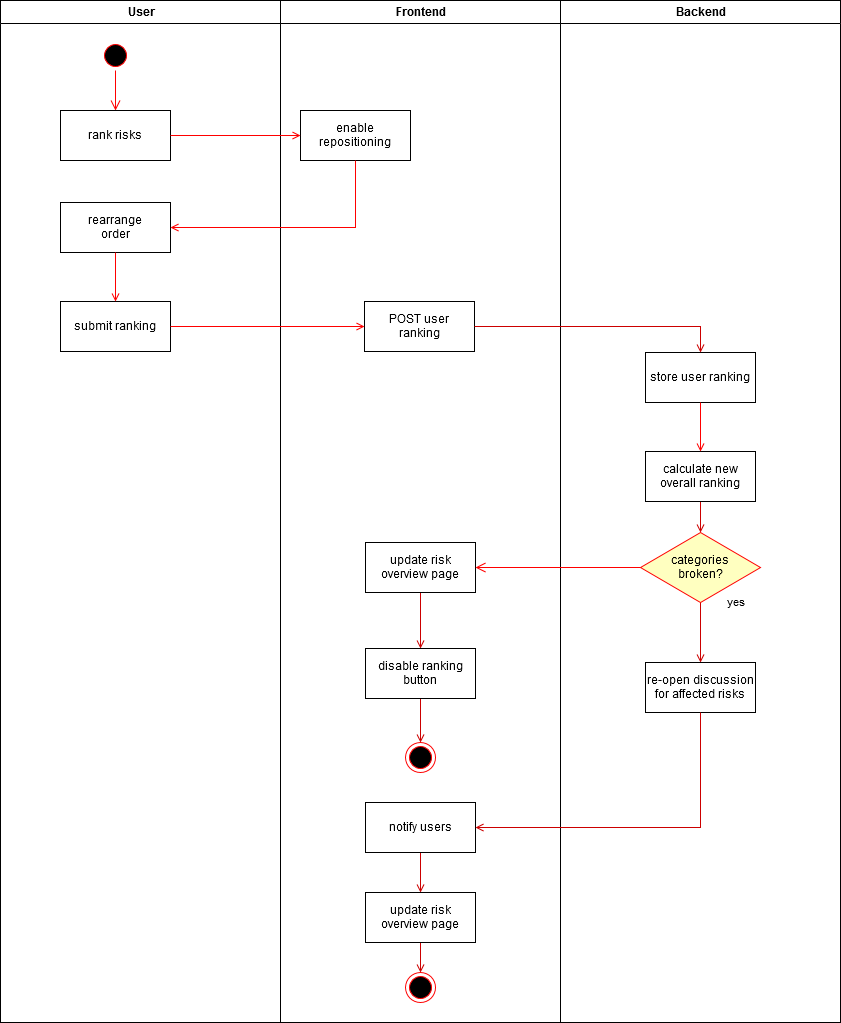
\includegraphics[width=0.8\textwidth]{Content/Domain/UC4RiskAdjustmentDiagram.png}
	\caption{Activity Diagram Use Case 4}
	\label{fig:label44}
\end{figure}

\paragraph*{Alternative Flows}\mbox{}\\

	The following steps will be added if the user enters the ranking process for the first time or has not participated in a ranking process for a prolonged period of time:
\begin{itemize}
	\vspace{-3mm}
	\setlength\itemsep{-1em}
	\item When the user presses the ranking button before the ranking mode is enabled an explation prompt will be shown.
	\item The user will be informed that they can submit their ranking only once.
	\item The user can either choose to confirm or they can choose that they do not want to be notified again doubling the time before the notification is shown again.
\end{itemize}
	
	The following steps will be added should the risk adjustment contradict the intital risk assesment:
\begin{itemize}
	\vspace{-3mm}
	\setlength\itemsep{-1em}
	\item A risk is ranked outside its category due to the average ranking process.
	\item The risk discussion on the risks which are now out of category is re-opened.
	\item The team members receive a notification to re-evaluate those risks.
\end{itemize}


\paragraph*{Special Requirements and Preconditions}\mbox{}\\
This use case has the following preconditions:
\begin{enumerate}
	\vspace{-3mm}
	\setlength\itemsep{-1em}
	\item The user is part of a project which contains risks.
	\item The initial risk discussion is finished.
	\item The user has either not yet ranked the risks or 
	\item the risk adjustment has been re-opened by the project manager.
\end{enumerate}

\paragraph*{Postconditions and Persistance}\mbox{}\\
The postconditions for this use case are:
\begin{enumerate}
	\vspace{-3mm}
	\setlength\itemsep{-1em}
	\item The risk order will be updated for all project members.
	\item The ranking option will be disabled until new risks are proposed or the ranking is manually reset by the project manager.
\noindent	
The ranking results are persisted in the database. The user ranking is transmitted to the backend via post request where the project risk ranking is handled accordingly.
\end{enumerate}


\newpage
% UC5 ====================================================
\subsubsection{Use Case Specification: \ac{UC}5 Risk Pool}
\label{sec:domainBbf}

\paragraph*{Description}\mbox{}\\
The risk pool serves to share knowledge among different teams and to store experiences. Users can vote for project risks to be added to the risk pool. After a certain quorum is reached the risk will be moved to the risk pool and will be persisted together with its responses there. Whenever a new risk is created the user will then have the option to check the pool risks if their risk is already present. They can then add a reference to the pool risks to their project risks. Pool risk can already have responses attached to them and will display the average occurrence probability and impact severity estimates of their project references giving an indication of how other teams evaluated the risk. The individual project risk evaluation process will still be undertaken for pool risks. \\
To remove risks from the risk pool a user will have to request a voting process on the pool risk. They can choose to either have the risk deleted (because it is outdated for example) or to merge it with another risk. All users will then be notified that a pool risk is up for discussion and will be invited to vote. If the vote is favorable the risk will be deleted and in case of a merge request its responses and references will be moved to the merge risk. \\
Quorums can be adjusted by project managers however there will be a notification that the change affects all teams and other project managers will receive a notification should a quorum be changed. 

\paragraph*{Screenshots}\mbox{}\\
Insert screenshots and shortly explain what can be seen
\begin{figure}[h] 
	\centering
	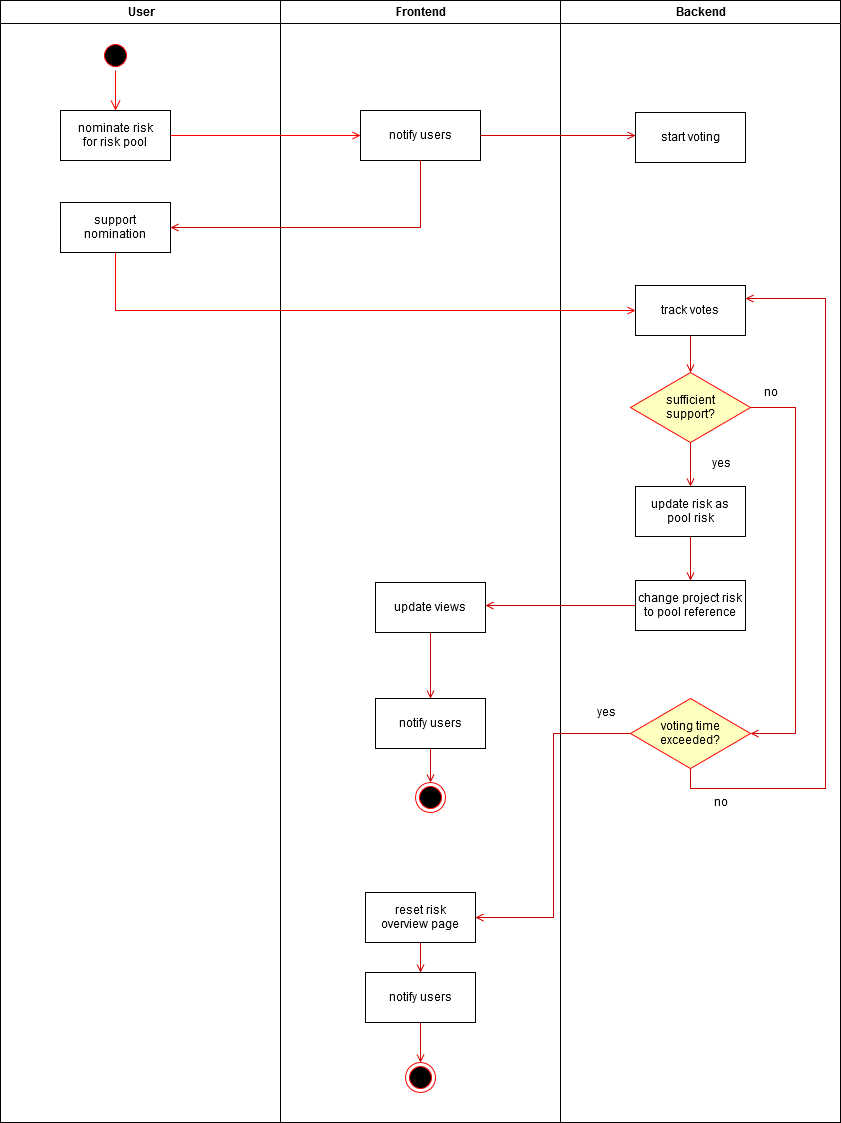
\includegraphics[width=0.1\textwidth]{Content/Domain/UC5RiskPoolDiagram.png}
	\caption{Use Case X: Detail}
	\label{fig:label5}
\end{figure}

\paragraph*{Basic Flow} \mbox{}\\
Add flow:
\begin{itemize}
	\vspace{-3mm}
	\setlength\itemsep{-1em}
	\item A user clicks on the "nominate for risk pool" button on a project risk's detail page.
	\item Other users on the project team will be notified that a risk has been nominated.
	\item The nomination button will be replaced by a support button for these users.
	\item Once a pre-defined quorum of users has supported the nomination the risk will be moved to the risk pool and the project risk will become a reference to the pool risk.
\end{itemize}

Remove flow:
\begin{itemize}
	\vspace{-3mm}
	\setlength\itemsep{-1em}
	\item A user nominates a pool risk for being removed on the pool risk's detail page.
	\item All users who are part of a project that references the pool risks will be notified.
	\item The nomination button will be replaced by a support button for those users.
	\item If a pre-defined quorum of users supports the nomination the project references will be turned into copies of the original risk and the copies risk will be removed from the risk pool.
\end{itemize}

Duplicate flow:
\begin{itemize}
	\vspace{-3mm}
	\setlength\itemsep{-1em}
	\item A user marks a pool risk as being a duplicate.
	\item The user will be shown a list of pool risks to mark the corresponding risk.
	\item All users which are part of projects that reference either risk will be notified.
	\item The nomination button will be replaced by a confirmation button for those users.
	\item If a pre-defined quorum of users confirms the duplication the risks will be merged.
	\item All references of the second risks will be redirected to the first, the response list will be merged and the duplicate will be deleted.
\end{itemize}

\subparagraph{Activity Diagram}\mbox{}\\
\begin{figure}[h]
	\centering
	
\includegraphics[width=0.1\textwidth]{Content/Domain/placeholder.png}
	\caption{Activity Diagram Use Case X}
	\label{fig:label55}
\end{figure}

\paragraph*{Alternative Flows}\mbox{}\\
The last steps of the above described flows will change if the quorum is not met within a pre-defined timeframe.
\begin{itemize}
	\vspace{-3mm}
	\setlength\itemsep{-1em}
	\item The risks will not be changed and the status from before the nomination will be restored.
\end{itemize}
	
\paragraph*{Special Requirements and Preconditions}\mbox{}\\
This use case has the following preconditions:
\begin{enumerate}
	\vspace{-3mm}
	\setlength\itemsep{-1em}
	\item The user is part of a project which contains risks.
	Or
	\item There is a risk in the risk pool.
	Or
	\item There are two similar risks in the risk pool.
\end{enumerate}

\paragraph*{Postconditions and Persistance}\mbox{}\\
The changes are instantly reflected in the database. Once the changes are confirmed corresponding PUT and DELETE requests update the database.

\newpage
% UC6 ====================================================
\subsubsection{Use Case Specification: \ac{UC}6 Risk Discussion}
\label{sec:domainBbg}

\paragraph*{Description}\mbox{}\\
The process of adding risks to a project is based on three steps:
\begin{enumerate}
	\vspace{-3mm}
	\setlength\itemsep{-1em}
	
	\item A project member proposes a risk (name and description). (UC3 Risk CRUD defined in chapter \ref{sec:domainBbd}).
	\item A specified number of project members review the proposed risk. After the review process the risk is ready for discussion.
	\item The whole project team discusses and defines:
	\begin{itemize}
		\vspace{-3mm}
		\setlength\itemsep{-1em}
		
		\item probability of occurence
		\item impact
		\item risk factor (defined by probability of occurence and impact)
		\item response(s)
		\item person in charge
	\end{itemize}
\end{enumerate}

\paragraph*{Screenshots}\mbox{}\\
tbd: Insert screenshots and shortly explain what can be seen
\begin{figure}[h] 
	\centering
	
\includegraphics[width=0.1\textwidth]{Content/Domain/placeholder.png}
	\caption{\ac{UC}6 Risk Discussion: TODO}
	\label{fig:label6}
\end{figure}

\newpage

\paragraph*{Basic Flow} \mbox{}\\

\begin{enumerate}
	\vspace{-3mm}
	\setlength\itemsep{-1em}
	
	\item A project member proposes a risk (name and description as defined in UC3 Risk CRUD chapter \ref{sec:domainBbd})
	\begin{itemize}
		\vspace{-3mm}
		\setlength\itemsep{-1em}
		
		\item The proposed risk is visible in the section proposed risks at the project overview page ("Proposed risks").
		\item All members of the project receive a notification (in their activity stream) about the new proposed risk and the request to review it.
	\end{itemize}
	
	\item A specified number of project members review the proposed risk. After the review process the risk is ready for discussion.
	\begin{itemize}
		\vspace{-3mm}
		\setlength\itemsep{-1em}
		
		\item When the specified number of project members have positively reviewed the risk, it is visible in the section ("Risks open to discussion").
		\item The project owner is able to manually start an estimation session for the risk (not recommended). The recommended way is to wait until a specified number of risks open for estimation are collected. Then an estimation session for all risks is automatically started.
	\end{itemize}
		
	\item The risk is estimated by the whole project team:
	\begin{itemize}
		\vspace{-3mm}
		\setlength\itemsep{-1em}
		
		\item All project members receive a notification (in their activity stream) to estimate the risk in terms of (probability of occurrence, impact) and to add response(s). Probability of occurrence and impact are mandatory fields, response(s) are optional.
		\item The risk factor is determined by the probability of occurrence and the impact.
		\item It is checked if at least one response is defined. If not the project members are notified to add a response.
		\item In the last step the person in charge is defined. Therefore a notification where the user is able to sign up for being responsible for the risk is sent to all project members.  
	\end{itemize}

	\item Finally the risk appears at the project risk table ("Project risks").
	
\end{enumerate}

\subparagraph{Activity Diagram}\mbox{}\\
\begin{figure}[!hp]
	\centering
	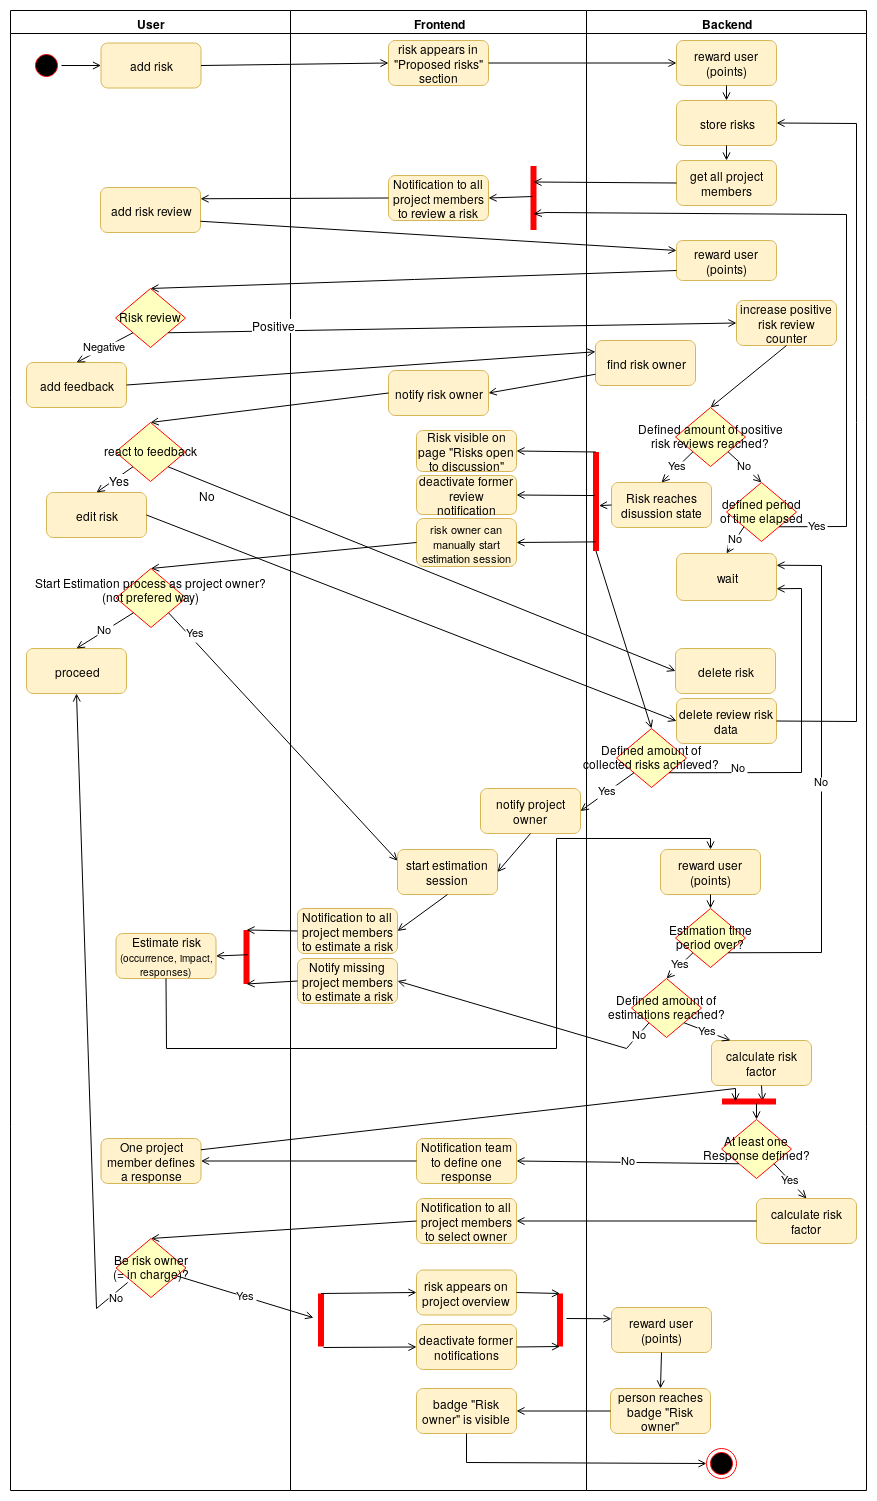
\includegraphics[width=0.8\textwidth]{Content/Domain/UC6RiskDiscussion.png}
	\caption{Activity Diagram \ac{UC}6 Risk Discussion}
	\label{fig:label66}
\end{figure}

\newpage

\paragraph*{Alternative Flows}\mbox{}\\

\noindent
Proposed risk receives negative reviews:
\begin{itemize}
	\vspace{-3mm}
	\setlength\itemsep{-1em}
	
	\item A project member negatively reviews a risk.
	\item The reviewing person adds feedback for the risk which is sent to the risk owner.
	\item The risk owner can edit or delete the proposed risk.
	\item When the risk is deleted it is removed from the section proposed risks.
	\item When the risk is edited the review process data is removed and the message for reviewing is sent again.
\end{itemize}

\noindent
Project members doesn't react to their notifications to:
\begin{enumerate}
	\vspace{-3mm}
	\setlength\itemsep{-1em}
	
	\item review a risk: When the needed amount of reviews is not achieved the notification is sent again.
	\item estimate a risk: When the needed amount of estimations is not achieved the notification is sent again.
	\item define a person in charge: When no person volunteers the notification is sent again. For finding a risk person in charge fast the Gamification concept Challenge is used.
\end{enumerate}

\paragraph*{Special Requirements and Preconditions}\mbox{}\\
The preconditions for this use case are:
\begin{enumerate}
	\vspace{-3mm}
	\setlength\itemsep{-1em}
	
	\item  A project exists.
	\item The user is member of the project.
	\item The user has proposed a risk.
\end{enumerate}

\paragraph*{Postconditions and Persistance}\mbox{}\\
The postconditions for this use case are:
\begin{enumerate}
	\vspace{-3mm}
	\setlength\itemsep{-1em}
	
	\item The proposed risk was reviewed and estimated. 
	\item The risk contains all relevant data.
	\item The risk is visible as part of the projects risk table.
\end{enumerate}

\newpage
% UC7 ====================================================
\subsubsection{Use Case Specification: \ac{UC}7 Risk Monitoring}
\label{sec:domainBbh}

\paragraph*{Description}\mbox{}\\
Describe the functionality

\paragraph*{Screenshots}\mbox{}\\
Insert screenshots and shortly explain what can be seen
\begin{figure}[h] 
	\centering
	
\includegraphics[width=0.1\textwidth]{Content/Domain/placeholder.png}
	\caption{Use Case X: Detail}
	\label{fig:label7}
\end{figure}

\paragraph*{Basic Flow} \mbox{}\\

Describe the most common path through this use case

\subparagraph{Activity Diagram}\mbox{}\\
\begin{figure}[h]
	\centering
	
\includegraphics[width=0.1\textwidth]{Content/Domain/placeholder.png}
	\caption{Activity Diagram Use Case X}
	\label{fig:label77}
\end{figure}

\paragraph*{Alternative Flows}\mbox{}\\
What can go wrong :D

\paragraph*{Special Requirements and Preconditions}\mbox{}\\
Where does the user come from, what does he have to do before he gets here

\paragraph*{Postconditions and Persistance}\mbox{}\\
What has changed and how do we make sure the change persists?

\newpage
% UC8 ====================================================
\subsubsection{Use Case Specification: \ac{UC}8 Risk Response Management}
\label{sec:domainBbi}

\paragraph*{Description}\mbox{}\\
Responses are ways to react to a risk. A new response can be added to a risk from the risk detail page. A response contains a name, a type and a description as well as the information whether the described steps have already been undertaken or not. Depending on the Type of risk a reminder can be set to remind the risk owner to repeat the response tasks.\\
The risk owner can remove a response on a project risk if the project manager concurs.\\
If the risk is a pool risk the response can also be a pool response. Pool responses can only be removed if all project managers who currently reference the risk concur. However, pool responses can be deactivated for the current project with only the current project manager agreeing to prevent situationally unsuitable response reminders.\\
A new response to a pool risk can be turned into a pool response via a voting process among team members.
This is a CRUD use case.

\paragraph*{Screenshots}\mbox{}\\
Insert screenshots and shortly explain what can be seen
\begin{figure}[h] 
	\centering
	
\includegraphics[width=0.1\textwidth]{Content/Domain/placeholder.png}
	\caption{Use Case X: Detail}
	\label{fig:label8}
\end{figure}

\paragraph*{Basic Flow} \mbox{}\\
\noindent
Creating a response:
\begin{itemize}
	\vspace{-3mm}
	\setlength\itemsep{-1.5em}
	\item When the user clicks the "+" button at the risk detail page in the response section.
	\item Then the screen for adding a new response is opened.
	\item When the response form is filled by the user.
	\item And the user clicks on the "Add response" button.
	\item Then the risk is synced with the server.
\end{itemize}

\spacing{1}
\noindent
Reading a response:
\begin{itemize}
	\vspace{-3mm}
	\setlength\itemsep{-1em}
	\item The user is on the risk detail site for a project risk.
	\item By clicking on a response a detail view is expanded.
	\item For exiting the detail view a minimize button is clicked.
\end{itemize}

\noindent
Updating a response: 
\begin{itemize}
	\vspace{-3mm}
	\setlength\itemsep{-1em}
	\item The user is on the risk detail site for a project risk.
	\item In the risk response section there is a pen button, which opens an editing form.
	\item By clicking the "Save" button the risk owner is notified of the changes.
	\item If the owner concurrs the changes are syncronized with the server.
\end{itemize} 

\noindent
Deleting a response:
\begin{itemize}
	\vspace{-3mm}
	\setlength\itemsep{-1em}
	\item The user is on the risk detail site for a project risks.
	\item By clicking a "Delete" button the project manager receives a notification.
	\item If the project manager concurrs the response is deleted.
\end{itemize}


\subparagraph{Activity Diagram}\mbox{}\\
\begin{figure}[h]
	\centering
	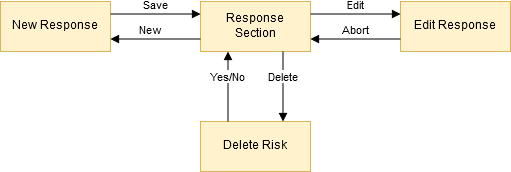
\includegraphics[[width=0.8\textwidth]{Content/Domain/UC8RiskResponseCRUDactivitydiagram}
	\caption{Activity Diagram Use Case 8}
	\label{fig:label88}
\end{figure}

\paragraph*{Alternative Flows}\mbox{}\\
In addition to the crud functionalities responses attached to a risk that references a pool risk can be nominated for becoming a pool response and thus being attached to pool risk permanently. The voting process is the same as for pool risk nomination described in UC 5\ref{sec:domainBbf}.
The update and delete flows change if the response is a pool response attached to a pool risk.
\begin{itemize}
	\vspace{-3mm}
	\setlength\itemsep{-1em}
	\item Updating a pool response requires project manager concurrance.
	\item Deleting a pool response will trigger a voting process as described in UC 5\ref{sec:domainBbf}. However it will be limited to project managers to prevent users from deleting unpleasant responses.
\end{itemize}


\paragraph*{Special Requirements and Preconditions}\mbox{}\\
The preconditions for this use case are:
\begin{enumerate}
	\vspace{-3mm}
	\setlength\itemsep{-1em}
	\item  A risk exists.
	\item The user is member of the project containing the risk.
	\item Deleting requires the user to also be the owner of the risk.
\end{enumerate}
For pool responses the following preconditions replace the above described:
\begin{enumerate}
	\vspace{-3mm}
	\setlength\itemsep{-1em}
	\item The response is attached to a pool risk.
\end{enumerate}

\paragraph*{Postconditions and Persistance}\mbox{}\\
Changes are directly reflected into the database via corresponding POST, PUT and DELETE requests.



TODO: INSERT USE CASES CONTEXT

\subsection{Requirements}
\label{sec:domainBc}
Couldn't find a better translation for "Anspruch" :/
Describes which 'Ansprüche' we have regarding the following categories:
\subsubsection{Usability}
\label{sec:domainBca}
\subsubsection{Reliability}
\label{sec:domainBcb}
\subsubsection{Performance}
\label{sec:domainBcc}
\subsubsection{Supportability}
\label{sec:domainBcd}

\subsection{Design Constraints}
\label{sec:domainBd}
Where does our software run? Where does it not? Which functions cannot be covered and why? Which conditions are required to use the software? Stuff like that

\subsection{Interfaces}
\label{sec:domainBe}
\subsubsection{User Interfaces}
\label{sec:domainBea}
Describe the views the software will have
\subsubsection{Further Interfaces}
\label{sec:domainBeb}
Software, Hardware and Communcation Interfaces... expand subsubsections if necessary
